% Three bits decide which UART is on the header, and a fourth state is
% what this bench actually had.
%
% Drawn here rather than copied from the vendor document. The facts come
% from BCM2835 ARM Peripherals, Broadcom, 6 February 2012: Table 6-1 on
% page 90 for the register address, Table 6-3 on page 92 for which bits
% belong to which pin, Table 6-2 on page 92 for the encoding, and Table
% 6-31 on page 102 with its legend on page 103 for what each alternate
% function is. Nothing from that document is reproduced; this is the same
% information redrawn to show one path through it.
%
% The point of the drawing: pins 8 and 10 are not "the UART". They are
% whichever UART a three bit field says, and their reset value is neither.
\documentclass[tikz, border=4pt]{standalone}
% Shared styles for the Project 9 figures.
%
% Every figure in this directory is standalone: it inputs this file and
% compiles on its own with
%
%     pdflatex arch.tex
%
% so a reader can render one drawing without building a book around it.
%
% The palette carries the distinction this project keeps confusing when it
% is drawn in one colour: what runs on the target, what runs on the host,
% and which of the two halves of the serial cable a given box is talking
% to. The fourth colour is for a fault that produces no symptom, which is
% three of the four faults here and the reason the project exists.
\usepackage{tikz}
\usepackage[siunitx]{circuitikz}
\usetikzlibrary{arrows.meta, backgrounds, calc, fit, positioning, shapes.geometric, shapes.misc}

\definecolor{usercol}{RGB}{222, 235, 247}   % target, user space
\definecolor{kerncol}{RGB}{198, 219, 239}   % target, kernel
\definecolor{hostcol}{RGB}{229, 245, 224}   % host, off the board
\definecolor{toolcol}{RGB}{254, 217, 118}   % a debugging tool
\definecolor{hwcol}{RGB}{229, 229, 229}     % hardware, files, RAM
\definecolor{quietcol}{RGB}{245, 245, 245}  % a fault with no symptom
\definecolor{linecol}{RGB}{70, 70, 70}
\definecolor{badcol}{RGB}{200, 60, 60}
\definecolor{okcol}{RGB}{60, 140, 70}

\tikzset{
  blk/.style   = {draw=linecol, rounded corners=2pt, align=center,
                  font=\sffamily\small, inner sep=4pt, minimum height=9mm},
  user/.style  = {blk, fill=usercol},
  kern/.style  = {blk, fill=kerncol},
  host/.style  = {blk, fill=hostcol},
  tool/.style  = {blk, fill=toolcol},
  hw/.style    = {blk, fill=hwcol},
  quiet/.style = {blk, fill=quietcol, draw=linecol!50, dashed},
  bad/.style   = {blk, fill=white, draw=badcol, thick, text=badcol},
  layer/.style = {draw=linecol!40, dashed, rounded corners=3pt, inner sep=6pt},
  layerlabel/.style = {font=\sffamily\scriptsize\bfseries, inner sep=2pt},
  lbl/.style   = {font=\sffamily\scriptsize, fill=white, inner sep=1pt},
  flow/.style  = {-{Stealth[length=2mm]}, draw=linecol, thick},
  bus/.style   = {{Stealth[length=2mm]}-{Stealth[length=2mm]}, draw=linecol,
                  thick},
  % The serial line is drawn thick and dark everywhere it appears, because
  % the single point of this project's host side is that it is one wire.
  wire/.style  = {{Stealth[length=2mm]}-{Stealth[length=2mm]}, draw=linecol,
                  very thick},
  % UML sequence
  actor/.style = {blk, fill=usercol, font=\sffamily\scriptsize,
                  minimum height=6mm},
  lifeline/.style = {draw=linecol!50, dashed},
  msg/.style   = {-{Stealth[length=1.6mm]}, draw=linecol},
  reply/.style = {-{Stealth[length=1.6mm]}, draw=linecol, dashed},
  umlnote/.style = {draw=linecol!60, fill=yellow!12, rounded corners=1pt,
                    font=\sffamily\scriptsize, align=left, inner sep=3pt},
  activation/.style = {draw=linecol, fill=usercol, minimum width=2mm},
  % decision tree
  qst/.style   = {draw=linecol, fill=white, diamond, aspect=2.6, align=center,
                  font=\sffamily\scriptsize, inner sep=1pt},
  ans/.style   = {font=\sffamily\scriptsize\itshape, inner sep=1pt},
  fix/.style   = {blk, fill=hostcol, font=\sffamily\scriptsize, align=left},
  trans/.style = {-{Stealth[length=1.6mm]}, draw=linecol},
  % fault matrix
  cell/.style  = {draw=linecol!40, minimum width=17mm, minimum height=7mm,
                  font=\sffamily\scriptsize, align=center},
  hit/.style   = {cell, fill=okcol!25},
  miss/.style  = {cell, fill=badcol!12, text=badcol},
  head/.style  = {cell, font=\sffamily\scriptsize\bfseries, fill=hwcol},
}


\begin{document}
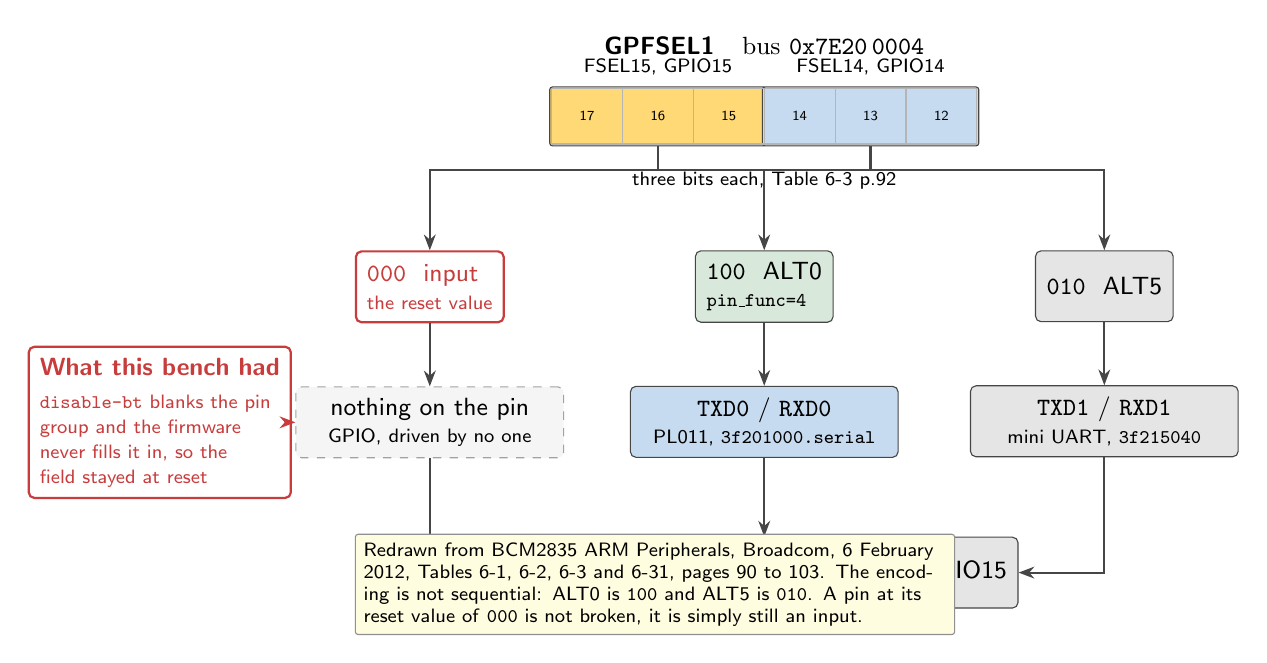
\begin{tikzpicture}[font=\sffamily\small]

  %% ---------------- the register ----------------
  \node[font=\sffamily\small\bfseries] (reghdr) at (0,0)
       {GPFSEL1\quad\normalfont\small bus \texttt{0x7E20\,0004}};

  % A strip of bit cells. Only the two fields that matter are coloured.
  \foreach \i/\x in {17/0, 16/1, 15/2, 14/3, 13/4, 12/5} {
    \node[cell, minimum width=9mm, minimum height=7mm]
         (b\i) at (\x*9mm - 22.5mm, -9mm) {\tiny \i};
  }
  \begin{scope}[on background layer]
    \node[fit=(b17)(b15), fill=toolcol, draw=linecol, rounded corners=1pt,
          inner sep=0.5pt] (f15) {};
    \node[fit=(b14)(b12), fill=kerncol, draw=linecol, rounded corners=1pt,
          inner sep=0.5pt] (f14) {};
  \end{scope}
  \node[lbl, anchor=south] at ($(f15.north)+(0,1mm)$) {FSEL15, GPIO15};
  \node[lbl, anchor=south] at ($(f14.north)+(0,1mm)$) {FSEL14, GPIO14};
  \node[font=\sffamily\scriptsize, anchor=north] at ($(f14.south)!0.5!(f15.south)+(0,-2mm)$)
       {three bits each, Table 6-3 p.92};

  %% ---------------- the three values ----------------
  \node[bad, align=left, anchor=north west] (v000)
       at (-52mm, -26mm) {\texttt{000}\ \ input\\[-1pt]
                          \scriptsize the reset value};
  \node[blk, fill=okcol!20, align=left, anchor=north] (v100)
       at (0mm, -26mm) {\texttt{100}\ \ ALT0\\[-1pt]
                        \scriptsize \texttt{pin\_func=4}};
  \node[blk, fill=hwcol, align=left, anchor=north east] (v010)
       at (52mm, -26mm) {\texttt{010}\ \ ALT5};

  \draw[flow] (f14.south) -- ++(0,-3mm) -| (v000.north);
  \draw[flow] (f14.south) -- ++(0,-3mm) -| (v100.north);
  \draw[flow] (f15.south) -- ++(0,-3mm) -| (v010.north);

  %% ---------------- what each one means ----------------
  \node[quiet, align=center, anchor=north, minimum width=34mm] (nowhere)
       at ($(v000.south)+(0,-8mm)$)
       {nothing on the pin\\[-1pt]\scriptsize GPIO, driven by no one};

  \node[kern, align=center, anchor=north, minimum width=34mm] (pl011)
       at ($(v100.south)+(0,-8mm)$)
       {\texttt{TXD0} / \texttt{RXD0}\\[-1pt]
        \scriptsize PL011, \texttt{3f201000.serial}};

  \node[hw, align=center, anchor=north, minimum width=34mm] (mini)
       at ($(v010.south)+(0,-8mm)$)
       {\texttt{TXD1} / \texttt{RXD1}\\[-1pt]
        \scriptsize mini UART, \texttt{3f215040}};

  \draw[flow] (v000) -- (nowhere);
  \draw[flow] (v100) -- (pl011);
  \draw[flow] (v010) -- (mini);

  %% ---------------- the pins ----------------
  \node[hw, align=center, anchor=north, minimum width=56mm] (pins)
       at ($(pl011.south)+(0,-10mm)$)
       {header \textbf{pin 8} = GPIO14 \quad \textbf{pin 10} = GPIO15};
  \draw[flow] (pl011) -- (pins);
  \draw[flow] (mini.south) |- ($(pins.east)+(6mm,0)$) -- (pins.east);
  \draw[flow] (nowhere.south) |- ($(pins.west)+(-6mm,0)$) -- (pins.west);

  %% ---------------- what the bench had ----------------
  \node[bad, align=left, anchor=west] (had)
       at ($(nowhere.west)+(-34mm,0)$)
       {\textbf{What this bench had}\\[1pt]
        \scriptsize \texttt{disable-bt} blanks the pin\\[-2pt]
        \scriptsize group and the firmware\\[-2pt]
        \scriptsize never fills it in, so the\\[-2pt]
        \scriptsize field stayed at reset};
  \draw[flow, draw=badcol] (had) -- (nowhere);

  \node[umlnote, anchor=north west, text width=74mm] at (-52mm, -62mm)
       {Redrawn from BCM2835 ARM Peripherals, Broadcom, 6 February 2012,
        Tables 6-1, 6-2, 6-3 and 6-31, pages 90 to 103. The encoding is
        not sequential: ALT0 is \texttt{100} and ALT5 is \texttt{010}.
        A pin at its reset value of \texttt{000} is not broken, it is
        simply still an input.};

\end{tikzpicture}
\end{document}
